
\section{Introducción}
El diseño, desarrollo, fabricación, armado, simulación y lanzamiento de cohetes, no es una tarea
sencilla ni repetida en intervalos de cortos de tiempo, al contrario, suelen llevar décadas y una
fuerte inversión para que sean posibles estos logros. El diseño y auge de vehículos VTVL viene
a subsanar estos factores ya que una vez terminada la misión el vehículo se puede reutilizar,
con mínimas intervenciones, y estaría listo para una nueva misión, atacando estos dos puntos principales anteriormente mencionados, el tiempo y el costo. Esto es a diferencia del método convencional donde el vehículo, luego de completar la misión, pasa a formar parte de basura espacial o, en el mejor de los casos, es recuperado del mar como el caso del Space Shuttle. 

\medskip

Los vehículos VTVL son tan viejos como el primer alunizaje. Traen en si varias ventajas frente a otros vehículos voladores como la gran reducción de espacio necesario para despegar y aterrizar. Esto no es un detalle menor dado que la mayor parte de la superficie terrestre de la tierra no son pistas de aterrizaje si no más bien terreno formado naturalmente.

\medskip

Este documento propone el diseño, simulación, control y fabricación de un vehículo con capacidades VTVL siendo un prototipo de baja escala. 
Este prototipo serviría como punta pie inicial
para vehículos de escala mayor que puedan completar misiones espaciales. Existen varias ventajas de implementar este tipo de tecnología.

\medskip

A baja escala, un vehículo que despega y aterriza por su cuenta, teniendo la capacidad de
superar obstáculos que se presenten, puede ser de gran utilidad en ambientes hostiles para el
ser humano, que esto se logre de manera rápida y efectiva podría ser la diferencia entre el
éxito o no de la misión.
Como ser el transporte de insumos médicos en tiempo real desde que un paciente lo requiere,
en zonas de acceso limitado.

\medskip

Últimamente hay un interés nuevo en imágenes espaciales. El vehículo podría ser utilizado para fines de sistemas de monitoreo y análisis geoespacial mediante el uso de estas imágenes, como hacen las empresas \textit{Ceres Imaging} y \textit{Satellogic}. %de una situación en la que no se disponga del tiempo suficiente para el accionar convencional a bajas velocidades como ser un helicóptero o un dron.  

\medskip

El vehículo una vez desarrollado y funcionando, puede servir de plataforma para diversos
estudios de fenómenos de dinámica de fluidos, como ser, mediciones aerodinámicas,
investigación del \textit{fuel sloshing} en vehículos con tanques esbeltos.

\medskip


Los sistemas de vehículos orbitales tienen sistemas complejos que deben ser testeados en una primera etapa mediante algún ensayo controlado. El vehículo que se desarrolla en el presente documento podría ser usado para tales fines como una plataforma para pruebas como ser el despliegue de una nariz o etapa, comprobación de sensores y actuadores a gran velocidad y con empuje variable.


\section{Estudios}
En lo que se refiere a la construcción del vehículo, el diseño propuesto paso por varias etapas y
decisiones de ingeniería hasta su forma final. Desde su diseño en lápiz y papel hasta la
simulación del CAD con el detalle del ultimo bulón del ensamble para poder recoger datos de
momentos de inercia, centros de masa y la dinámica del vehículo.

\subsection{Agua como propelente}\label{ssec:propAgua}
El primer prototipo muy distante del diseño final perteneciente a este trabajo, consistía en un
recipiente a presión con agua, abulonado a un chasis, con un gimbal y actuadores para poder redirigir el
empuje. 

\medskip

La figura \ref{fig:bottlerocket} muestra los resultados de una simulación de un vehículo pequeño de aluminio con un recipiente a presión lleno en parte de agua y aire a 200 bar. La simulación considera masa variable y una transición isoentrópica del gas en el recipiente. En el mejor de los casos se llegaba a un tiempo de vuelo cercano a los 4 segundos que no es suficiente para comprobar un sistema de control. 

Para optimizar este problema se modificaba

\begin{itemize}
    \item Diámetro de la tobera -- más empuje vs. menos tiempo de vuelo controlado
    \item Volumen de agua -- más tiempo de vuelo vs. mayor peso de vehículo
\end{itemize}


\begin{figure}[!ht]
    \centering
    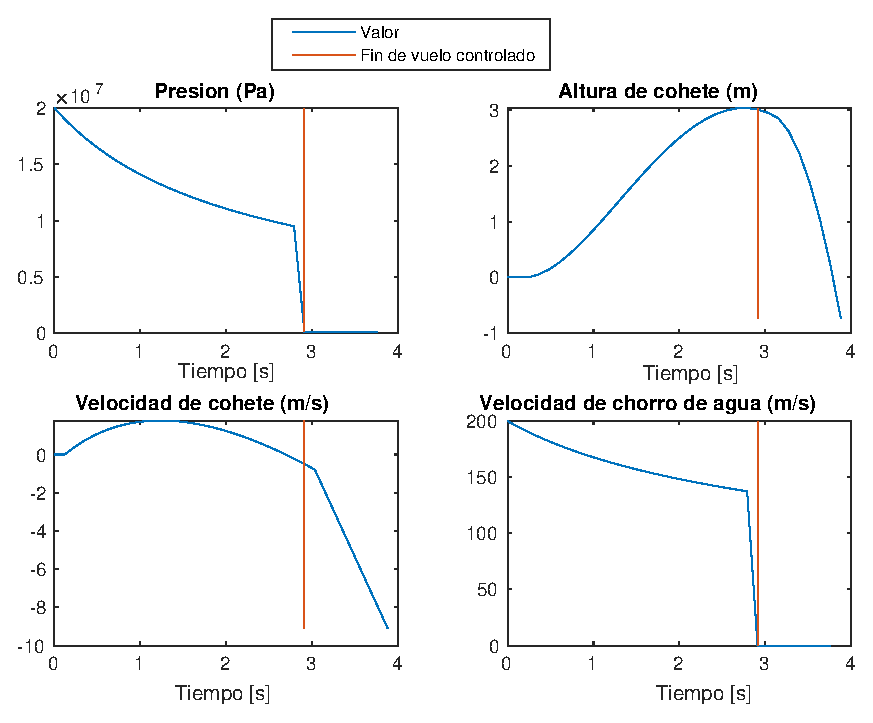
\includegraphics[width=0.8\linewidth]{fig/bottlerocket}
    \caption{Análisis preliminar para un vehículo propulsado por agua a presión. La presión es la del tanque (absoluta). El peso estructural que se utilizó fue de 10kg.}
    \label{fig:bottlerocket}
\end{figure}

\subsection{Turbina}\label{ssec:turbina}
Se propuso la construcción de una turbina de combustible líquido, como método de propulsión
del vehículo favorable debido al excelente cociente de peso-empuje.

Esta idea se vio descartada por la pandemia que estamos atravesando (COVID19) debido a que
no teníamos acceso al taller de la institución para poder realizar en tiempo y forma el
dispositivo mecánico, que era la primer tarea inmediata a tener en banco de pruebas
asegurando su funcionamiento en optimas condiciones, para luego proseguir con el desarrollo
del vehículo y el sistema de control.


\subsection{Propulsión eléctrica} \label{ssec:propelectrica}


\begin{figure}[htb]
    \centering
    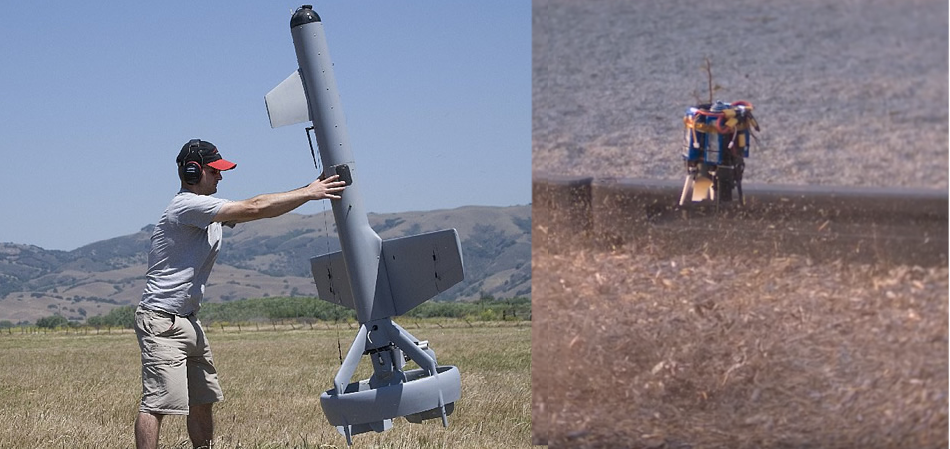
\includegraphics[width=0.8\linewidth]{fig/vbat_icarus.png}
    \caption{Dos vehículos VTVL eléctricos modernos. ``VBat'' (Izq.) y ``\href{https://hackaday.com/2018/08/31/single-rotor-drone-a-thrust-vectoring-monocopter/}{Ikarus}'' (Der.).}
    \label{fig:vbat_icarus}
\end{figure}

Luego de descartar las ideas vistas en \ref{ssec:propAgua} y \ref{ssec:turbina} se pasó al análisis de la incorporación de una turbina eléctrica que es un dispositivo ya existente en el mercado, no en nuestro país, pero que podría llegar a importarse mediante una
inversión privada.\footnote{Agradecemos a \gls{lia} por hacerse cargo de la compra de todos los elementos necesarios para la fabricación del cohete.} Dado el alcance de un proyecto de universidad se decidió por un diseño compuesto por elementos comercialmente disponibles.\footnote{\textit{Commercial off the shelf} (COTS)}


\medskip


Para lograr estas tareas generalmente los vehículos VTVL de baja escala generalmente son propulsados por motores eléctricos.

\medskip

Los vehículos VTVL eléctricos son propulsados por hélices en su mayoría y constan casi siempre de 3 o más propulsores en un arreglo simétrico y plano. Recientemente hay un interés por la construcción de vehículos de una sola hélice por la buena relación empuje--peso que tienen. Sin embargo, estos vehículos no vienen sin sus complicaciones: 

\begin{itemize}
    \item La rotación dada al aire por la hélice causa un momento en el eje de propulsión que es contrarrestado en vehículos multirrotores.
    \item Inclinar al rotor durante su funcionamiento causa una fuerza perpendicular a la dirección de inclinación conocido como el efecto giroscópico. 
\end{itemize}

El primer punto es mitigado fácilmente agregando álabes a la salida del chorro para enderezar el flujo y contrarrestar la rotación. El segundo punto solo se resuelve conociendo las ecuaciones de momento angular y controlando actuadores con un sistema de control a lazo cerrado. Los sistemas vistos en la figura \ref{fig:vbat_icarus} tienen la particularidad de poder ser representados con relativa facilidad usando un solo marco de referencia inercial para el cálculo de las ecuaciones de momento angular.

Existen placas pre-programadas para vehículos multirrotores, pero en el caso de vehículos monorrotores de hélice fija se precisa re-programar la placa para compensar por el efecto giroscópico y agregar dinámica de álabes ya que no existe software disponible aún para esta configuración. En el caso de tener una hélice móvil se suma un nivel de complejidad agregada debido al despeje de las ecuaciones de momento angular (ver sección \ref{sec:ecuacionesRigid}). Al momento de escribir este documento aún no hay desarrollo disponible de carácter público para esta configuración.